\documentclass{standalone}
\usepackage{tikz}
\usepackage{hsbcommon}
\begin{document}
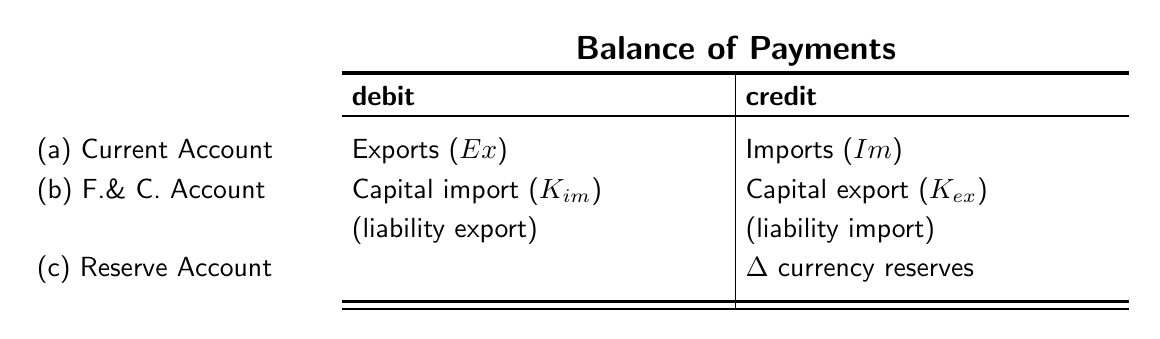
\begin{tikzpicture}
\tikzset{every node/.append style={font=\sffamily}}

    \begin{scope}[y=3ex] %% T
        \node at (0,0.6) {\large\textbf{Balance of Payments}};
        \draw[ultra thick] (-5,0) -- (5,0);
        
        \draw[thick] (-5,-1.2) -- (5,-1.2);
        \node[anchor=north west] at (-5,-0.1) {\textbf{debit}};
        \node[anchor=north west] at (0,-0.1) {\textbf{credit}};

    \end{scope}


%% debit 



    \foreach [count=\i] \myaccount/\mydebit/\mycredit in 
    {
        (a) Current Account/Exports ($Ex$)/Imports ($Im$),
        (b) F.\& C. Account/Capital import ($K_{im}$)/ Capital export ($K_{ex}$),
            /(liability export)/(liability import),
        (c) Reserve Account/ / $\Delta$ currency reserves
    }
    {
        \node[anchor=west] at (-9,-0.5*\i-0.5) {\myaccount};
        \node[anchor=west] at (-5,-0.5*\i-0.5) {\mydebit};
        \node[anchor=west] at (0,-0.5*\i-0.5) {\mycredit};
        \coordinate (last) at (-5,-0.5*\i-1);
    }
    
% %% credit

%     \foreach [count=\i] \myposition in 
%     {
%         Financial Account,
%         -- direct Investment,
%         -- portfolio Investment,
%         \hspace{2em}-- bonds,
%         \hspace{2em}-- savings,
%         \hspace{2em}-- equities,
%         -- Other investment,
%         Capital Account,
%         -- capital transfers,
%         -- immaterial asset transfers,
%         Reserve Account (currency)
%     }
%     {
%         \coordinate (last) at (0,-0.5*\i-1);
%     }

    \draw[] (0,0) -- (0, |- last);
    \draw[thick] (-5, |- last) -- (5, |- last);
    \draw[thick] ([shift=({0,0.1})] -5, |- last) -- ([shift=({0,0.1})] 5, |- last);
    
\end{tikzpicture}
\end{document}
